%% 
\documentclass{article}

\usepackage[tmargin=1in,bmargin=1in,lmargin=1in,rmargin=1in]{geometry}

\usepackage{amsthm}
\usepackage{amsmath}
\usepackage{amssymb}
\usepackage{graphicx}


\newtheorem{assumption}{Assumption}

%\makeatletter
%%%%%%%%%%%%%%%%%%%%%%%%%%%%%% Textclass specific LaTeX commands.
\theoremstyle{plain}
\newtheorem{thm}{\protect\theoremname}
\theoremstyle{remark}
\newtheorem{rem}{\protect\remarkname}
\theoremstyle{definition}
\newtheorem{problem}{\protect\problemname}
\theoremstyle{plain}
\newtheorem{lem}{\protect\lemmaname}
\theoremstyle{plain}
\newtheorem{cor}{\protect\corollaryname}


%\makeatother

\providecommand{\corollaryname}{Corollary}
\providecommand{\lemmaname}{Lemma}
\providecommand{\problemname}{Problem}
\providecommand{\remarkname}{Remark}
\providecommand{\theoremname}{Theorem}

\begin{document}

\title{COM S 578X: Optimization for Machine Learning \\
Homework 1}
\author{Name: \qquad{}Email: }
\maketitle


\begin{problem}
% You could type the problem here, or leave it blank if you only want to generate the numbering.
\end{problem}

Let $x=[r,\upsilon,\varphi,\omega]^{T}$. The nonlinear system can
be reformulated in the form of $\dot{x}=f(x)+g(x)u$, where 
\[
f(x)=\left[\begin{array}{c}
\upsilon\\
-g\sin\varphi+r\omega^{2}\\
\omega\\
-\frac{2mr\upsilon\omega}{J+mr^{2}}-\frac{mgr\cos\varphi}{J+mr^{2}}
\end{array}\right],\ g(x)=\left[\begin{array}{c}
0\\
0\\
0\\
1
\end{array}\right].
\]


Tracking errors of coordinate $z$ are shown in Fig. \ref{fig:TCze0}. 

Other symbols $\mathbb{R}$, $\mathbb{Q}$, $\mathbb{Z}$, $\cos$,
and $\sin$. 

\begin{thm}
If $f$ is absolutely continuous, then $\dot{f}(t)$=g(t) almost everywhere in the sense of Lebesgue measure.
\end{thm}

\begin{assumption}
If $f$ is absolutely continuous, then $\dot{f}(t)$=g(t) almost everywhere in the sense of Lebesgue measure.
\end{assumption}

\begin{rem}
If $f$ is absolutely continuous, then $\dot{f}(t)$=g(t) almost everywhere in the sense of Lebesgue measure.
\end{rem}

\begin{problem}
If $f$ is absolutely continuous, then $\dot{f}(t)$=g(t) almost everywhere in the sense of Lebesgue measure.
\end{problem}

\begin{lem}
If $f$ is absolutely continuous, then $\dot{f}(t)$=g(t) almost everywhere in the sense of Lebesgue measure.
\end{lem}

\begin{cor}
If $f$ is absolutely continuous, then $\dot{f}(t)$=g(t) almost everywhere in the sense of Lebesgue measure.
\end{cor}

\begin{proof}
Here is my important proof
\end{proof}

\begin{center}
\begin{figure}
\begin{centering}
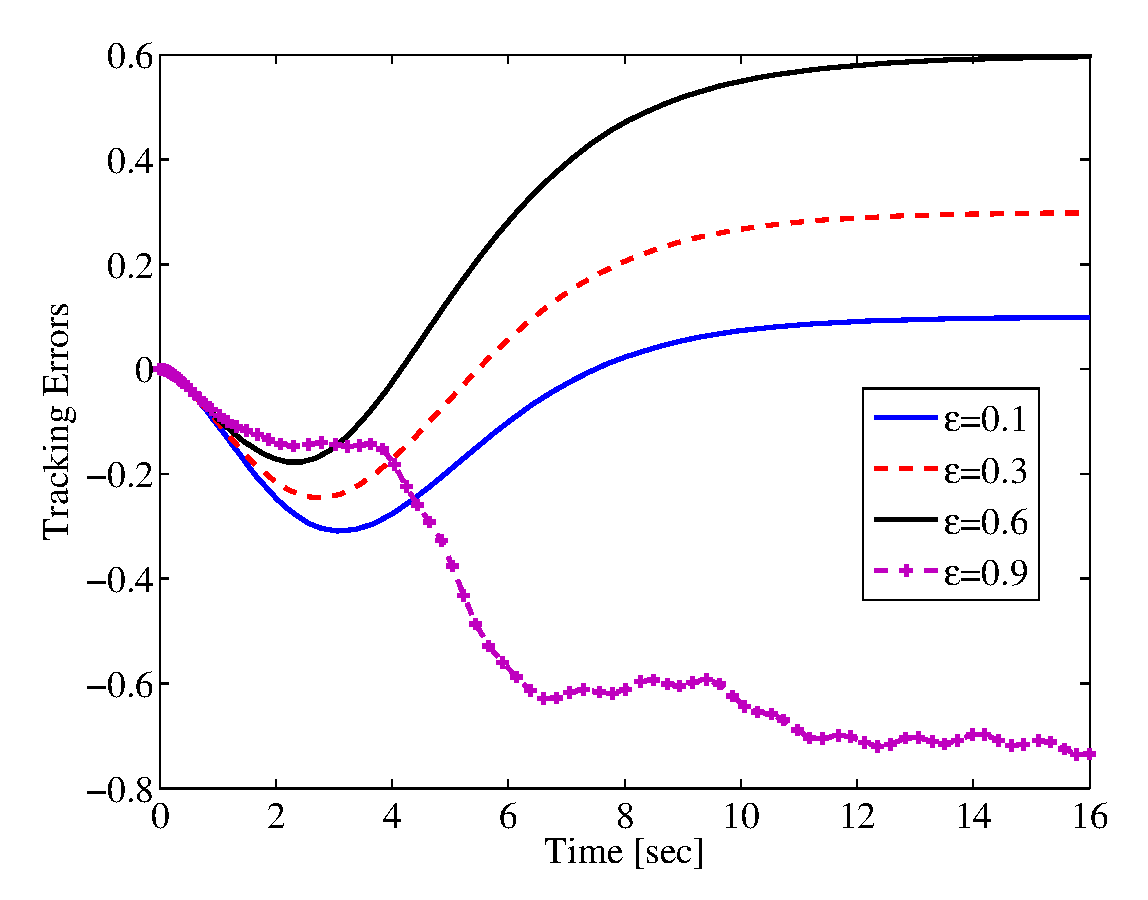
\includegraphics[clip,width=0.6\linewidth]{name}
\end{centering}
\centering{}\caption{\label{fig:TCze0}Tracking errors of the $z$ coordinate with different
$\varepsilon$}
\end{figure}
\end{center}

\end{document}
